

\tikzset{every picture/.style={line width=0.75pt}} %set default line width to 0.75pt        

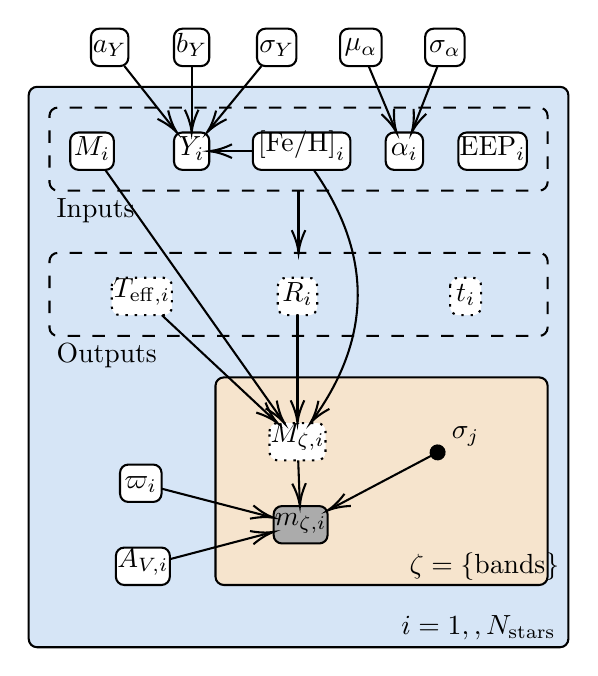
\begin{tikzpicture}[x=0.75pt,y=0.75pt,yscale=-1,xscale=1]
%uncomment if require: \path (0,384); %set diagram left start at 0, and has height of 384

%Shape: Rectangle [id:dp010165550931289014] 
\draw   (50,70) -- (70,70) -- (70,90) -- (50,90) -- cycle ;
%Shape: Rectangle [id:dp9376205267267221] 
\draw  [fill={rgb, 255:red, 214; green, 229; blue, 246 }  ,fill opacity=1 ] (30,54) .. controls (30,51.79) and (31.79,50) .. (34,50) -- (286,50) .. controls (288.21,50) and (290,51.79) .. (290,54) -- (290,316) .. controls (290,318.21) and (288.21,320) .. (286,320) -- (34,320) .. controls (31.79,320) and (30,318.21) .. (30,316) -- cycle ;
%Shape: Rectangle [id:dp0879962430090866] 
\draw  [dash pattern={on 4.5pt off 4.5pt}] (40,134) .. controls (40,131.79) and (41.79,130) .. (44,130) -- (276,130) .. controls (278.21,130) and (280,131.79) .. (280,134) -- (280,166) .. controls (280,168.21) and (278.21,170) .. (276,170) -- (44,170) .. controls (41.79,170) and (40,168.21) .. (40,166) -- cycle ;
%Shape: Rectangle [id:dp4207868301071993] 
\draw   (150,210) -- (170,210) -- (170,230) -- (150,230) -- cycle ;
%Shape: Rectangle [id:dp10030238688422877] 
\draw   (150,250) -- (170,250) -- (170,270) -- (150,270) -- cycle ;
%Shape: Rectangle [id:dp8355634642427261] 
\draw   (230,230) -- (250,230) -- (250,250) -- (230,250) -- cycle ;
%Shape: Rectangle [id:dp5906205088171197] 
\draw  [fill={rgb, 255:red, 246; green, 228; blue, 205 }  ,fill opacity=1 ] (120,194) .. controls (120,191.79) and (121.79,190) .. (124,190) -- (276,190) .. controls (278.21,190) and (280,191.79) .. (280,194) -- (280,286) .. controls (280,288.21) and (278.21,290) .. (276,290) -- (124,290) .. controls (121.79,290) and (120,288.21) .. (120,286) -- cycle ;
%Straight Lines [id:da4973220211869567] 
\draw    (160,100) -- (160,128) ;
\draw [shift={(160,130)}, rotate = 270] [color={rgb, 255:red, 0; green, 0; blue, 0 }  ][line width=0.75]    (10.93,-3.29) .. controls (6.95,-1.4) and (3.31,-0.3) .. (0,0) .. controls (3.31,0.3) and (6.95,1.4) .. (10.93,3.29)   ;
%Shape: Rectangle [id:dp5690927935939454] 
\draw  [dash pattern={on 4.5pt off 4.5pt}] (40,64) .. controls (40,61.79) and (41.79,60) .. (44,60) -- (276,60) .. controls (278.21,60) and (280,61.79) .. (280,64) -- (280,96) .. controls (280,98.21) and (278.21,100) .. (276,100) -- (44,100) .. controls (41.79,100) and (40,98.21) .. (40,96) -- cycle ;

% Text Node
\draw  [fill={rgb, 255:red, 255; green, 255; blue, 255 }  ,fill opacity=1 ][line width=0.75]   (138,76) .. controls (138,73.79) and (139.79,72) .. (142,72) -- (181,72) .. controls (183.21,72) and (185,73.79) .. (185,76) -- (185,86) .. controls (185,88.21) and (183.21,90) .. (181,90) -- (142,90) .. controls (139.79,90) and (138,88.21) .. (138,86) -- cycle  ;
\draw (161.5,86.8) node [anchor=south] [inner sep=0.75pt]   [align=left] {$\displaystyle \mathrm{[ Fe/H]}_{i}$};
% Text Node
\draw  [fill={rgb, 255:red, 255; green, 255; blue, 255 }  ,fill opacity=1 ][line width=0.75]   (50,76) .. controls (50,73.79) and (51.79,72) .. (54,72) -- (67,72) .. controls (69.21,72) and (71,73.79) .. (71,76) -- (71,86) .. controls (71,88.21) and (69.21,90) .. (67,90) -- (54,90) .. controls (51.79,90) and (50,88.21) .. (50,86) -- cycle  ;
\draw (60.5,86.8) node [anchor=south] [inner sep=0.75pt]   [align=left] {$\displaystyle M_{i}$};
% Text Node
\draw  [fill={rgb, 255:red, 255; green, 255; blue, 255 }  ,fill opacity=1 ][line width=0.75]   (237,76) .. controls (237,73.79) and (238.79,72) .. (241,72) -- (266,72) .. controls (268.21,72) and (270,73.79) .. (270,76) -- (270,86) .. controls (270,88.21) and (268.21,90) .. (266,90) -- (241,90) .. controls (238.79,90) and (237,88.21) .. (237,86) -- cycle  ;
\draw (253.5,86.8) node [anchor=south] [inner sep=0.75pt]   [align=left] {$\displaystyle \mathrm{EEP}_{i}$};
% Text Node
\draw  [fill={rgb, 255:red, 255; green, 255; blue, 255 }  ,fill opacity=1 ][line width=0.75]   (100,76) .. controls (100,73.79) and (101.79,72) .. (104,72) -- (113,72) .. controls (115.21,72) and (117,73.79) .. (117,76) -- (117,86) .. controls (117,88.21) and (115.21,90) .. (113,90) -- (104,90) .. controls (101.79,90) and (100,88.21) .. (100,86) -- cycle  ;
\draw (108.5,86.8) node [anchor=south] [inner sep=0.75pt]   [align=left] {$\displaystyle Y_{i}$};
% Text Node
\draw  [fill={rgb, 255:red, 255; green, 255; blue, 255 }  ,fill opacity=1 ][line width=0.75]   (202,76) .. controls (202,73.79) and (203.79,72) .. (206,72) -- (216,72) .. controls (218.21,72) and (220,73.79) .. (220,76) -- (220,86) .. controls (220,88.21) and (218.21,90) .. (216,90) -- (206,90) .. controls (203.79,90) and (202,88.21) .. (202,86) -- cycle  ;
\draw (211,86.8) node [anchor=south] [inner sep=0.75pt]   [align=left] {$\displaystyle \alpha _{i}$};
% Text Node
\draw  [fill={rgb, 255:red, 255; green, 255; blue, 255 }  ,fill opacity=1 ][dash pattern={on 0.84pt off 2.51pt}]  (70,146) .. controls (70,143.79) and (71.79,142) .. (74,142) -- (95,142) .. controls (97.21,142) and (99,143.79) .. (99,146) -- (99,156) .. controls (99,158.21) and (97.21,160) .. (95,160) -- (74,160) .. controls (71.79,160) and (70,158.21) .. (70,156) -- cycle  ;
\draw (84.5,156.8) node [anchor=south] [inner sep=0.75pt]   [align=left] {$\displaystyle T_{\mathrm{eff} ,i}$};
% Text Node
\draw  [fill={rgb, 255:red, 255; green, 255; blue, 255 }  ,fill opacity=1 ][dash pattern={on 0.84pt off 2.51pt}]  (233,146) .. controls (233,143.79) and (234.79,142) .. (237,142) -- (244,142) .. controls (246.21,142) and (248,143.79) .. (248,146) -- (248,156) .. controls (248,158.21) and (246.21,160) .. (244,160) -- (237,160) .. controls (234.79,160) and (233,158.21) .. (233,156) -- cycle  ;
\draw (240.5,156.8) node [anchor=south] [inner sep=0.75pt]   [align=left] {$\displaystyle t_{i}$};
% Text Node
\draw  [fill={rgb, 255:red, 255; green, 255; blue, 255 }  ,fill opacity=1 ][dash pattern={on 0.84pt off 2.51pt}]  (150,146) .. controls (150,143.79) and (151.79,142) .. (154,142) -- (165,142) .. controls (167.21,142) and (169,143.79) .. (169,146) -- (169,156) .. controls (169,158.21) and (167.21,160) .. (165,160) -- (154,160) .. controls (151.79,160) and (150,158.21) .. (150,156) -- cycle  ;
\draw (159.5,156.8) node [anchor=south] [inner sep=0.75pt]   [align=left] {$\displaystyle R_{i}$};
% Text Node
\draw  [fill={rgb, 255:red, 255; green, 255; blue, 255 }  ,fill opacity=1 ]  (74,236) .. controls (74,233.79) and (75.79,232) .. (78,232) -- (90,232) .. controls (92.21,232) and (94,233.79) .. (94,236) -- (94,246) .. controls (94,248.21) and (92.21,250) .. (90,250) -- (78,250) .. controls (75.79,250) and (74,248.21) .. (74,246) -- cycle  ;
\draw (84,246.8) node [anchor=south] [inner sep=0.75pt]   [align=left] {$\displaystyle \varpi _{i}$};
% Text Node
\draw  [fill={rgb, 255:red, 255; green, 255; blue, 255 }  ,fill opacity=1 ]  (72,276) .. controls (72,273.79) and (73.79,272) .. (76,272) -- (94,272) .. controls (96.21,272) and (98,273.79) .. (98,276) -- (98,286) .. controls (98,288.21) and (96.21,290) .. (94,290) -- (76,290) .. controls (73.79,290) and (72,288.21) .. (72,286) -- cycle  ;
\draw (85,286.8) node [anchor=south] [inner sep=0.75pt]   [align=left] {$\displaystyle A_{V,i}$};
% Text Node
\draw  [fill={rgb, 255:red, 171; green, 171; blue, 171 }  ,fill opacity=1 ]  (148,256) .. controls (148,253.79) and (149.79,252) .. (152,252) -- (170,252) .. controls (172.21,252) and (174,253.79) .. (174,256) -- (174,266) .. controls (174,268.21) and (172.21,270) .. (170,270) -- (152,270) .. controls (149.79,270) and (148,268.21) .. (148,266) -- cycle  ;
\draw (161,266.8) node [anchor=south] [inner sep=0.75pt]   [align=left] {$\displaystyle m_{\zeta ,i}$};
% Text Node
\draw  [fill={rgb, 255:red, 255; green, 255; blue, 255 }  ,fill opacity=1 ][dash pattern={on 0.84pt off 2.51pt}]  (146,216) .. controls (146,213.79) and (147.79,212) .. (150,212) -- (169,212) .. controls (171.21,212) and (173,213.79) .. (173,216) -- (173,226) .. controls (173,228.21) and (171.21,230) .. (169,230) -- (150,230) .. controls (147.79,230) and (146,228.21) .. (146,226) -- cycle  ;
\draw (159.5,226.8) node [anchor=south] [inner sep=0.75pt]   [align=left] {$\displaystyle M_{\zeta ,i}$};
% Text Node
\draw (240.5,224.8) node [anchor=south] [inner sep=0.75pt]  [color={rgb, 255:red, 0; green, 0; blue, 0 }  ,opacity=1 ] [align=left] {$\displaystyle \sigma _{j}$};
% Text Node
\draw  [fill={rgb, 255:red, 255; green, 255; blue, 255 }  ,fill opacity=1 ][line width=0.75]   (60,26) .. controls (60,23.79) and (61.79,22) .. (64,22) -- (74,22) .. controls (76.21,22) and (78,23.79) .. (78,26) -- (78,36) .. controls (78,38.21) and (76.21,40) .. (74,40) -- (64,40) .. controls (61.79,40) and (60,38.21) .. (60,36) -- cycle  ;
\draw (69,36.8) node [anchor=south] [inner sep=0.75pt]   [align=left] {$\displaystyle a_{Y}$};
% Text Node
\draw  [fill={rgb, 255:red, 255; green, 255; blue, 255 }  ,fill opacity=1 ][line width=0.75]   (100,26) .. controls (100,23.79) and (101.79,22) .. (104,22) -- (113,22) .. controls (115.21,22) and (117,23.79) .. (117,26) -- (117,36) .. controls (117,38.21) and (115.21,40) .. (113,40) -- (104,40) .. controls (101.79,40) and (100,38.21) .. (100,36) -- cycle  ;
\draw (108.5,36.8) node [anchor=south] [inner sep=0.75pt]   [align=left] {$\displaystyle b_{Y}$};
% Text Node
\draw  [fill={rgb, 255:red, 255; green, 255; blue, 255 }  ,fill opacity=1 ][line width=0.75]   (140,26) .. controls (140,23.79) and (141.79,22) .. (144,22) -- (155,22) .. controls (157.21,22) and (159,23.79) .. (159,26) -- (159,36) .. controls (159,38.21) and (157.21,40) .. (155,40) -- (144,40) .. controls (141.79,40) and (140,38.21) .. (140,36) -- cycle  ;
\draw (149.5,36.8) node [anchor=south] [inner sep=0.75pt]   [align=left] {$\displaystyle \sigma _{Y}$};
% Text Node
\draw  [fill={rgb, 255:red, 255; green, 255; blue, 255 }  ,fill opacity=1 ][line width=0.75]   (180,26) .. controls (180,23.79) and (181.79,22) .. (184,22) -- (196,22) .. controls (198.21,22) and (200,23.79) .. (200,26) -- (200,36) .. controls (200,38.21) and (198.21,40) .. (196,40) -- (184,40) .. controls (181.79,40) and (180,38.21) .. (180,36) -- cycle  ;
\draw (190,36.8) node [anchor=south] [inner sep=0.75pt]   [align=left] {$\displaystyle \mu _{\alpha }$};
% Text Node
\draw  [fill={rgb, 255:red, 255; green, 255; blue, 255 }  ,fill opacity=1 ][line width=0.75]   (221,26) .. controls (221,23.79) and (222.79,22) .. (225,22) -- (236,22) .. controls (238.21,22) and (240,23.79) .. (240,26) -- (240,36) .. controls (240,38.21) and (238.21,40) .. (236,40) -- (225,40) .. controls (222.79,40) and (221,38.21) .. (221,36) -- cycle  ;
\draw (230.5,36.8) node [anchor=south] [inner sep=0.75pt]   [align=left] {$\displaystyle \sigma _{\alpha }$};
% Text Node
\draw (208,303.2) node [anchor=north west][inner sep=0.75pt]   [align=left] {$\displaystyle i=1,\dotsc ,N_{\mathrm{stars}}$};
% Text Node
\draw (212,273.2) node [anchor=north west][inner sep=0.75pt]   [align=left] {$\displaystyle \zeta =\{\mathrm{bands}\}$};
% Text Node
\draw (42,102.2) node [anchor=north west][inner sep=0.75pt]   [align=left] {Inputs};
% Text Node
\draw (42,172.2) node [anchor=north west][inner sep=0.75pt]   [align=left] {Outputs};
% Connection
\draw    (108.5,40) -- (108.5,70) ;
\draw [shift={(108.5,72)}, rotate = 270] [color={rgb, 255:red, 0; green, 0; blue, 0 }  ][line width=0.75]    (10.93,-3.29) .. controls (6.95,-1.4) and (3.31,-0.3) .. (0,0) .. controls (3.31,0.3) and (6.95,1.4) .. (10.93,3.29)   ;
% Connection
\draw    (76.11,40) -- (100.15,70.43) ;
\draw [shift={(101.39,72)}, rotate = 231.69] [color={rgb, 255:red, 0; green, 0; blue, 0 }  ][line width=0.75]    (10.93,-3.29) .. controls (6.95,-1.4) and (3.31,-0.3) .. (0,0) .. controls (3.31,0.3) and (6.95,1.4) .. (10.93,3.29)   ;
% Connection
\draw    (142.12,40) -- (117.15,70.45) ;
\draw [shift={(115.88,72)}, rotate = 309.35] [color={rgb, 255:red, 0; green, 0; blue, 0 }  ][line width=0.75]    (10.93,-3.29) .. controls (6.95,-1.4) and (3.31,-0.3) .. (0,0) .. controls (3.31,0.3) and (6.95,1.4) .. (10.93,3.29)   ;
% Connection
\draw    (193.78,40) -- (206.45,70.16) ;
\draw [shift={(207.22,72)}, rotate = 247.22] [color={rgb, 255:red, 0; green, 0; blue, 0 }  ][line width=0.75]    (10.93,-3.29) .. controls (6.95,-1.4) and (3.31,-0.3) .. (0,0) .. controls (3.31,0.3) and (6.95,1.4) .. (10.93,3.29)   ;
% Connection
\draw    (226.99,40) -- (215.24,70.14) ;
\draw [shift={(214.51,72)}, rotate = 291.31] [color={rgb, 255:red, 0; green, 0; blue, 0 }  ][line width=0.75]    (10.93,-3.29) .. controls (6.95,-1.4) and (3.31,-0.3) .. (0,0) .. controls (3.31,0.3) and (6.95,1.4) .. (10.93,3.29)   ;
% Connection
\draw    (138,81) -- (119,81) ;
\draw [shift={(117,81)}, rotate = 360] [color={rgb, 255:red, 0; green, 0; blue, 0 }  ][line width=0.75]    (10.93,-3.29) .. controls (6.95,-1.4) and (3.31,-0.3) .. (0,0) .. controls (3.31,0.3) and (6.95,1.4) .. (10.93,3.29)   ;
% Connection
\draw    (159.5,160) -- (159.5,210) ;
\draw [shift={(159.5,212)}, rotate = 270] [color={rgb, 255:red, 0; green, 0; blue, 0 }  ][line width=0.75]    (10.93,-3.29) .. controls (6.95,-1.4) and (3.31,-0.3) .. (0,0) .. controls (3.31,0.3) and (6.95,1.4) .. (10.93,3.29)   ;
% Connection
\draw    (94.14,160) -- (148.4,210.64) ;
\draw [shift={(149.86,212)}, rotate = 223.03] [color={rgb, 255:red, 0; green, 0; blue, 0 }  ][line width=0.75]    (10.93,-3.29) .. controls (6.95,-1.4) and (3.31,-0.3) .. (0,0) .. controls (3.31,0.3) and (6.95,1.4) .. (10.93,3.29)   ;
% Connection
\draw    (66.86,90) -- (151.98,210.37) ;
\draw [shift={(153.14,212)}, rotate = 234.73] [color={rgb, 255:red, 0; green, 0; blue, 0 }  ][line width=0.75]    (10.93,-3.29) .. controls (6.95,-1.4) and (3.31,-0.3) .. (0,0) .. controls (3.31,0.3) and (6.95,1.4) .. (10.93,3.29)   ;
% Connection
\draw    (167.33,90) .. controls (195.82,130.74) and (195.58,171) .. (166.59,210.79) ;
\draw [shift={(165.7,212)}, rotate = 306.62] [color={rgb, 255:red, 0; green, 0; blue, 0 }  ][line width=0.75]    (10.93,-3.29) .. controls (6.95,-1.4) and (3.31,-0.3) .. (0,0) .. controls (3.31,0.3) and (6.95,1.4) .. (10.93,3.29)   ;
% Connection
\draw    (227,226.13) -- (175.77,253.2) ;
\draw [shift={(174,254.13)}, rotate = 332.15] [color={rgb, 255:red, 0; green, 0; blue, 0 }  ][line width=0.75]    (10.93,-3.29) .. controls (6.95,-1.4) and (3.31,-0.3) .. (0,0) .. controls (3.31,0.3) and (6.95,1.4) .. (10.93,3.29)   ;
\draw [shift={(227,226.13)}, rotate = 152.15] [color={rgb, 255:red, 0; green, 0; blue, 0 }  ][fill={rgb, 255:red, 0; green, 0; blue, 0 }  ][line width=0.75]      (0, 0) circle [x radius= 3.35, y radius= 3.35]   ;
% Connection
\draw    (159.84,230) -- (160.59,250) ;
\draw [shift={(160.66,252)}, rotate = 267.85] [color={rgb, 255:red, 0; green, 0; blue, 0 }  ][line width=0.75]    (10.93,-3.29) .. controls (6.95,-1.4) and (3.31,-0.3) .. (0,0) .. controls (3.31,0.3) and (6.95,1.4) .. (10.93,3.29)   ;
% Connection
\draw    (94,243.6) -- (146.06,257.12) ;
\draw [shift={(148,257.62)}, rotate = 194.56] [color={rgb, 255:red, 0; green, 0; blue, 0 }  ][line width=0.75]    (10.93,-3.29) .. controls (6.95,-1.4) and (3.31,-0.3) .. (0,0) .. controls (3.31,0.3) and (6.95,1.4) .. (10.93,3.29)   ;
% Connection
\draw    (98,277.58) -- (146.07,264.93) ;
\draw [shift={(148,264.42)}, rotate = 165.26] [color={rgb, 255:red, 0; green, 0; blue, 0 }  ][line width=0.75]    (10.93,-3.29) .. controls (6.95,-1.4) and (3.31,-0.3) .. (0,0) .. controls (3.31,0.3) and (6.95,1.4) .. (10.93,3.29)   ;

\end{tikzpicture}
